% !TeX spellcheck = en_GB

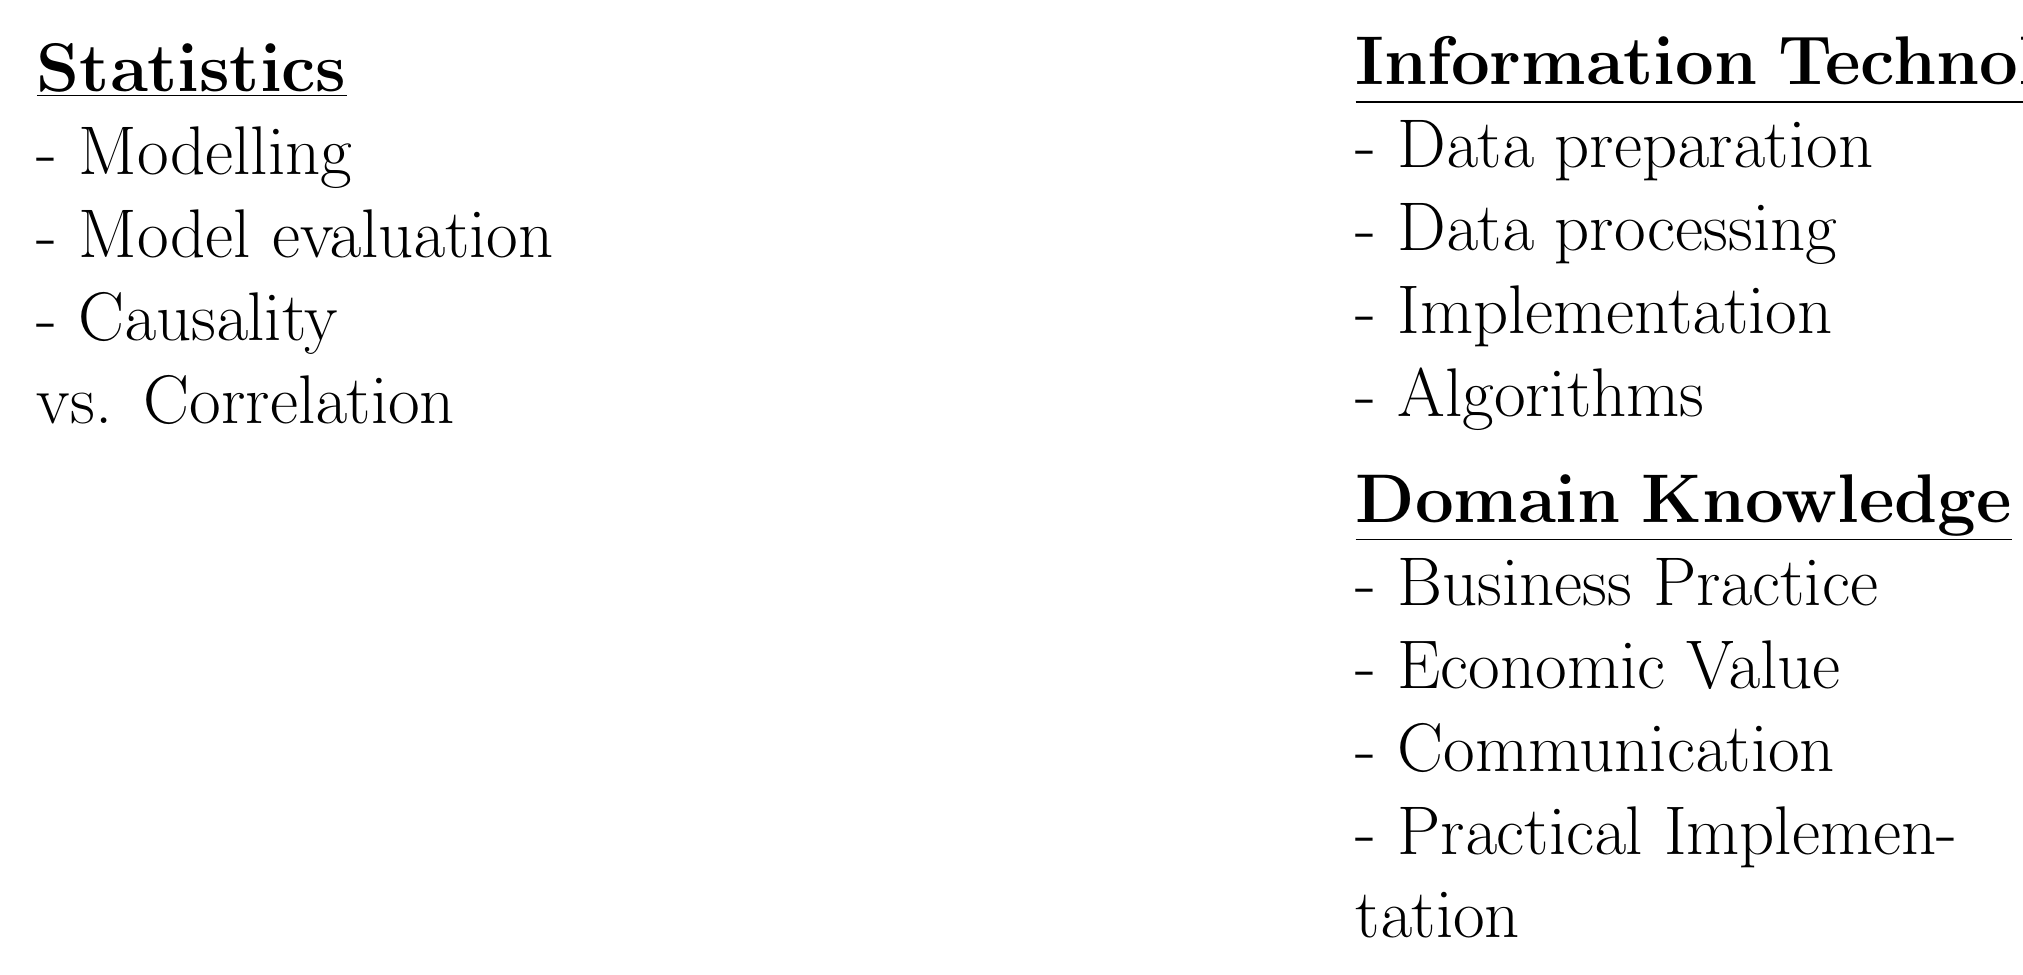
\begin{tikzpicture}[every node/.style={font=\Huge}]

	% Draw the pie chart with separated slices
	\pie[explode=0.3, text=inside, radius=4.5, hide number]{
		33.3/Information \\ Technology,
		33.3/Statistics,
		33.3/Domain \\ Knowledge
	}
	
	% Add legends or annotations
	\node[align=left, anchor=west, text width=7cm] at (5, 3) {
		\underline{\textbf{Information Technology}}\\
		- Data preparation\\
		- Data processing\\
		- Implementation\\
		- Algorithms
	};
	
	\node[align=left, anchor=east, text width=8cm] at (-3.5, 3) {
		\underline{\textbf{Statistics}}\\
		- Modelling\\
		- Model evaluation\\
		- Causality \\ vs. Correlation
	};
	
	\node[align=left, anchor=west, text width=8cm] at (5, -3) {
		\underline{\textbf{Domain Knowledge}}\\
		- Business Practice\\
		- Economic Value\\
		- Communication\\
		- Practical Implementation
	};
\end{tikzpicture}